% !TEX encoding = UTF-8 Unicode
\documentclass[a4paper]{article}

\usepackage{color}
\usepackage{url}
\usepackage[utf8]{inputenc} % make weird characters work
\usepackage{graphicx}
%\usepackage[nottoc]{tocbibind}

\usepackage[serbian, english]{babel}

\usepackage[unicode]{hyperref}
\hypersetup{colorlinks,citecolor=green,filecolor=green,linkcolor=blue,urlcolor=blue}

% used for code
\usepackage{color}
\usepackage{listings}
\usepackage{setspace}

\definecolor{Background}{rgb}{0.97,0.97,0.97}

\renewcommand{\lstlistingname}{Code}
\lstdefinelanguage{Python3}{
	language=Python,
	firstnumber=1,
	stepnumber=1,
	numbers=left,
	numbersep=5pt, 
	tabsize=4,
	basicstyle=\small\ttfamily,	
	morekeywords={import,from,class,def,for,while,if,is,in,elif,else,not,and,or,print,break,
		continue,return,True,False,None,access,as,,del,except,exec,finally,global,import,lambda,pass,print,raise,try,assert},
	stringstyle=\color{mymauve},
	commentstyle=\color{mygreen},  
	keywordstyle=\color{blue},
	backgroundcolor=\color{Background},	
	captionpos=b,  
	frame=single,	  
 	breakatwhitespace=false,
 	breaklines=true,
 	escapeinside={\%*}{*)},
 	extendedchars=true,
 	keepspaces=true,
	numberstyle=\tiny\color{mygray},
  	rulecolor=\color{black},
  	showspaces=false,
  	showstringspaces=false,
  	showtabs=false,
}

% this will be used when we want to show results
\lstdefinelanguage{Print}{
	numbers=none,
	tabsize=4,
	basicstyle=\small\ttfamily,
	frame=none	
}

\definecolor{mygreen}{rgb}{0,0.6,0}
\definecolor{mygray}{rgb}{0.5,0.5,0.5}
\definecolor{mymauve}{rgb}{0.58,0,0.82}

\lstset{ 
                  % show the filename of files included with \lstinputlisting; also try caption instead of title
}

\begin{document}

\title{Mining NBA}
\author{David Gavrilović}
% \date{9.~april 2015.}
\maketitle
\thispagestyle{empty}

\newpage

\tableofcontents
\thispagestyle{empty}

\newpage

\section{Stats 101}
\label{Stats_101}

\subsection{Traditional stats}
\label{Traditional_stats}


\begin{itemize}
	\item \textbf{Pos} - Position. Traditionaly, position can be one of the following: \textit{\textbf{PG}} - point guard, \textit{\textbf{SG}} - shooting guard, \textit{\textbf{SF}} - small forward, \textit{\textbf{PF}} - power forward and \textit{\textbf{C}} - center. Nowdays, one player usually plays multiple positions and usually is one of the: \textit{\textbf{Point}} - primarly PG, \textit{\textbf{Combo guard}} - plays PG and SG, \textit{\textbf{Wing}} - SF and SG, \textit{\textbf{Forward}} - PF and SF, \textit{\textbf{Big}} - usually C but can also be PF.
	\item \textbf{G} - Games. Number of games player played in during a season.
	\item \textbf{GS} - Games started. Number of games player started. Cannot be greater than G.
	\item \textbf{MP} - Minutes played (Per game or total in a season).
	\item \textbf{FG} - Field goals.
	\item \textbf{FGA} - Field goals attempts.
	\item \textbf{FG\%} - Field goal percentage. Calculated as FG / FGA.
	\item \textbf{3P} - 3-point field goals.
	\item \textbf{3PA} - 3-point field goal attempts.
	\item \textbf{3P\%} - 3-point percentage. Calculated as 3P / 3PA.
	\item \textbf{2P} - 2-point field goals. 
	\item \textbf{2PA} - 2-point field goal attempts.
	\item \textbf{2P\%} - 2-point percentage. Calculated as 2P / 2PA.
	\item \textbf{FT} - Free throws.
	\item \textbf{FTA} - Free throw attempts.
	\item \textbf{FT\%} - Free throws percentage. Calculated as FT / FTA.
	\item \textbf{eFG\%} - Field goal percentage that takes into account that a 3-point field goal is, by one point, worth more than a 2-point field goal. Calculated as (FG + 0.5 * 3P) / FGA.
	\item \textbf{ORB} - Offensive rebounds.
	\item \textbf{TRB} - Defensive rebounds.
	\item \textbf{AST} - Assists.
	\item \textbf{STL} - Steals.
	\item \textbf{BLK} - Blocks.
	\item \textbf{TOV} - Turnovers.
	\item \textbf{PF} - Personal fouls.
	\item \textbf{PTS or PPG} - Points or Points per game.	
\end{itemize}	
	
\subsection{Advanced stats}
\label{Advanced_stats}

\begin{itemize}
	\item \textbf{ORtg} - Offensive rating. An estimate of points produced/scored by a player/team per 100 possessions \cite{odrt}.
	\item \textbf{DRtg} - Defensive rating. An estimate of point allowed per 100 possessions \cite{odrt}.  
	\item \textbf{PER} - Player efficiency rating. A measure of a per minute production standardized such that the league average is 15 \cite{per}.
	\item \textbf{TS\%} - True shooting percentage. Points per scoring attempt converted to the 2-point field goal percentage needed to score that many points per attempt. Calculated as  PTS / (2 *  FGA + 0.44 * FTA). 
	\item \textbf{3PAr} - 3-Point attempt rate. Percentage of FGA from 3-point range.
	\item \textbf{FTr} - Free throw attempt rate. Number of FTA per FGA.
	\item \textbf{ORD\%} - Offensive rebound percentage. An estimate of the percentage of available offensive rebounds a player grabbed while he was on the floor.
	\item \textbf{DRB\%} - Defensive rebound percentage. An estimate of the percentage of available defensive rebounds a player grabbed while he was on the floor
	\item \textbf{TRB\%} - Total rebound percentage. An estimate of the percentage of available rebounds a player grabbed while he was on the floor. 
	\item \textbf{AST\%} - Assist percentage. An estimate of the percentage of teammate field goals a player assisted while he was on the floor.
	\item \textbf{STL\%} - Steal Percentage. An estimate of the percentage of opponent possessions that end with a steal by the player while he was on the floor. 
	\item \textbf{BLK\%} - Block percentage. An estimate of the percentage of opponent two-point field goal attempts blocked by the player while he was on the floor. 
	\item \textbf{TOV\%} - Turnover percentage. An estimate of turnovers per 100 plays. 
	\item \textbf{USG\%} - Usage percentage. An estimate of the percentage of team plays used by a player while he was on the floor.  
	\item \textbf{OWS} - Offensive win shares. An estimate of the number of wins contributed by a player due to his offense \cite{ws}. 
	\item \textbf{DWS} - Defensive win shares. An estimate of the number of wins contributed by a player due to his defense \cite{ws}. 
	\item \textbf{WS} - Win shares. An estimate number of wins contibuted by a player \cite{ws}.
	\item \textbf{WS/48} - Win shares per 48 minutes. League average is around 0.100.
	\item \textbf{OBPM} - Offensive Box plus/minus. A box score estimate of the offensive points per 100 possessions that a player contributed above a league-average player, translated to an average team \cite{bpm}.
	\item \textbf{DBPM} - Defensive Box plus/minus. A box score estimate of the defensive points per 100 possessions that a player contributed above a league-average player, translated to an average team \cite{bpm}.
	\item \textbf{BPM} - Box plus/minus. A box score estimate of the points per 100 possessions that a player contributed above a league-average player, translated to an average team \cite{bpm}.
	\item \textbf{VORP} - Value over replacement player. An estimate of the points per 100 team possessions that a player contributed above a replacement-level (-2.0) player, translated to an average team and prorated to an 82-game season \cite{bpm}.

\end{itemize}

\section{Calculating prime of an average player}
\label{prime}

In this section we will try to determine when does an average player hit their \textit{prime}. But first, what is prime? In order to answer that question we must first define something called \textit{peak}. Peak is the best season player had in his career. Knowing that, prime can be defined as player's seasons in which he is close, or somewhat close, to his peak. Knowing length of a player's prime is important, because prime is probably the most important thing when discussing player's career. \\

In this paper only individual statistics will be used in process of estimating prime years of a player. Because the ultimate stat that can correctly measure when do players hit their prime does not exist (yet), multiple other stats will be used, both traditional and advanced. Those stats are, mostly, PTS, FG and FGA from traditional and PER, WS/48, BPM and VORP from advanced stats. Reasoning behind first three is, well, player in his prime should be best version of himself, so he will probably score and shoot more than in his non-prime seasons. Stats such as PER, BPM and VORP exist so we could determine impact on a game by player, or how good a player is. Prime season should have higher values for this stat than for other seasons. WS per 48 is used to determine players contribution to winning, per 48 minutes, the lenght of a game without overtime. It's also expected for this stat to be higher for seasons in player's prime than for the other seasons. \\  

Of course, different players can hit their prime at different age. Let's check prime years od some of the players inducted, or soon to be inducted, into the Naismith memorial basketball hall of fame. Selected players are chosen without any particular reason. Players used are Bird \ref{plt:bird}, Shaq \ref{plt:shaq} and Duncan \ref{plt:duncan}. As we can see from the shown box plots, mentioned players have the best stats when they were around 26 to 30 years old. From that we can conclude that that was the lenght of their prime.  \\


\begin{figure}[h!]
\begin{center}
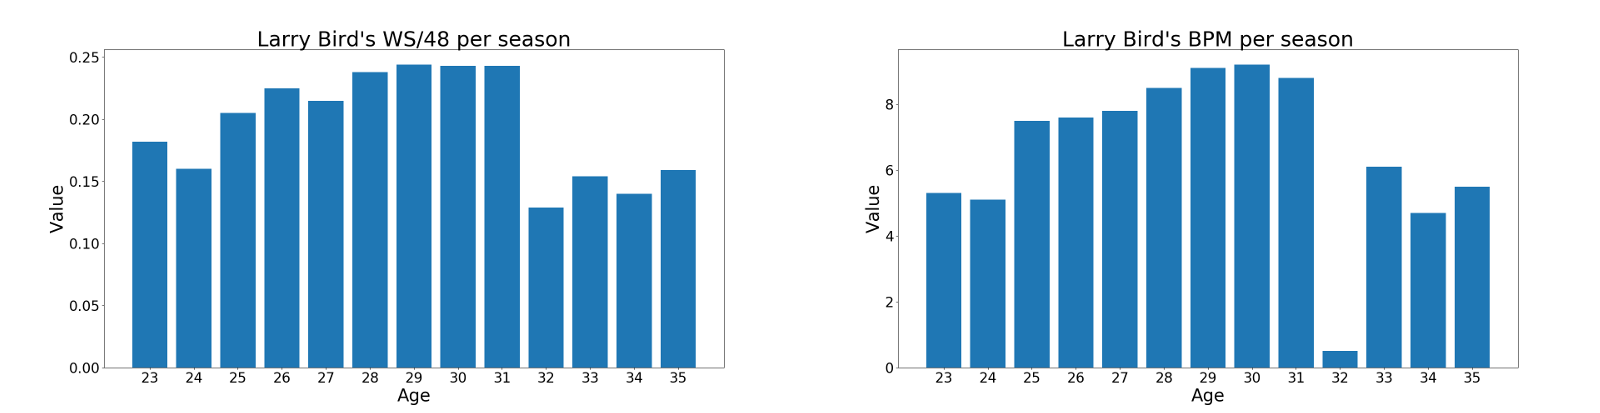
\includegraphics[scale=0.32]{bird.png}
\end{center}
\caption{Bird's WS/48 and BPM per season}
\label{plt:bird}
\end{figure}

\begin{figure}[h!]
\begin{center}
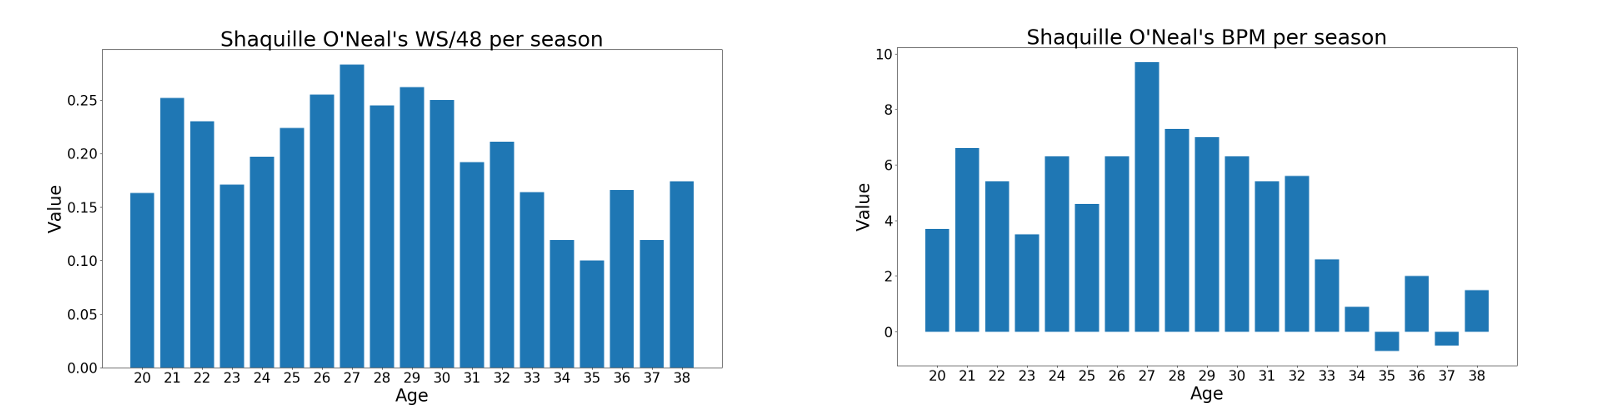
\includegraphics[scale=0.32]{shaq.png} % 2 x 800px and 413px
\end{center}
\caption{Shaq's WS/48 and BPM per season}
\label{plt:shaq}
\end{figure}

\begin{figure}[h!]
\begin{center}
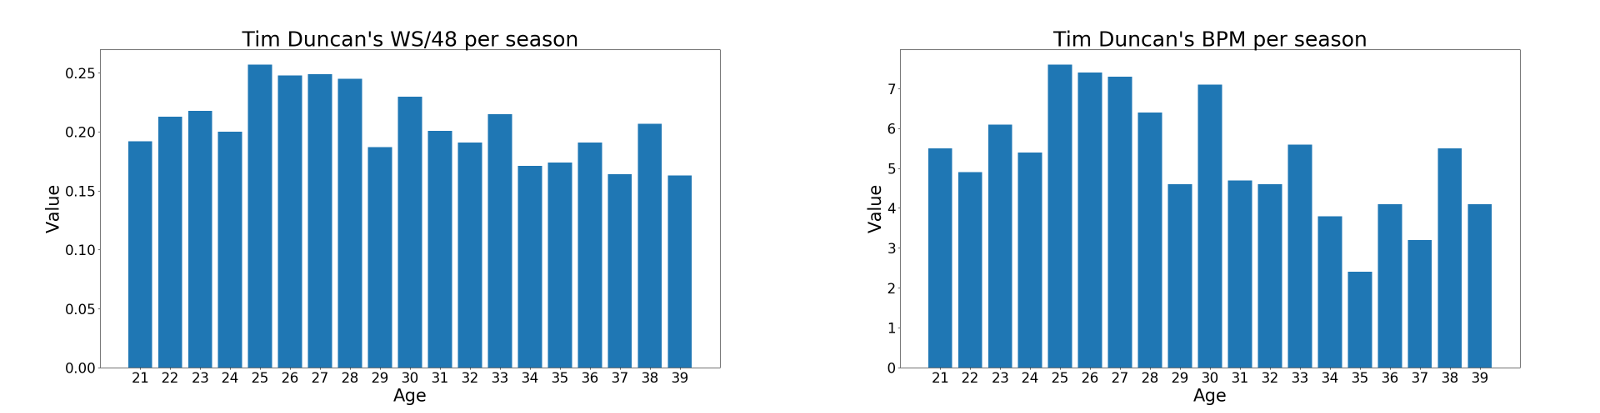
\includegraphics[scale=0.32]{duncan.png}
\end{center}
\caption{Duncan's WS/48 and BPM per season}
\label{plt:duncan}
\end{figure}


In the next step of determining prime of players, I checked at what age do players win awards, such as \textit{regular season MVP}, \textit{FMVP}, \textit{DPOY} and \textit{Sixth man of the year}. Plots are shown in figure \ref{plt:awards}. Every plot but plot for Sixth man of the year is somewhat similar. The number of awards players won while in their late twenties and eary thirties is greater than number of awards in other years. Defensive player of the year award plot is different, where players aged from 23 to 31 won with roughly the same frequency, with an exception of players who were 28 years old when they won, and the ones who were 27. After that there is a significant drop. These plots are showing us that the best players in the season are usually ones between 26 and 31 years old. But those players are stars and superstars. What about an average player?  \\

\begin{figure}[h!]
\begin{center}
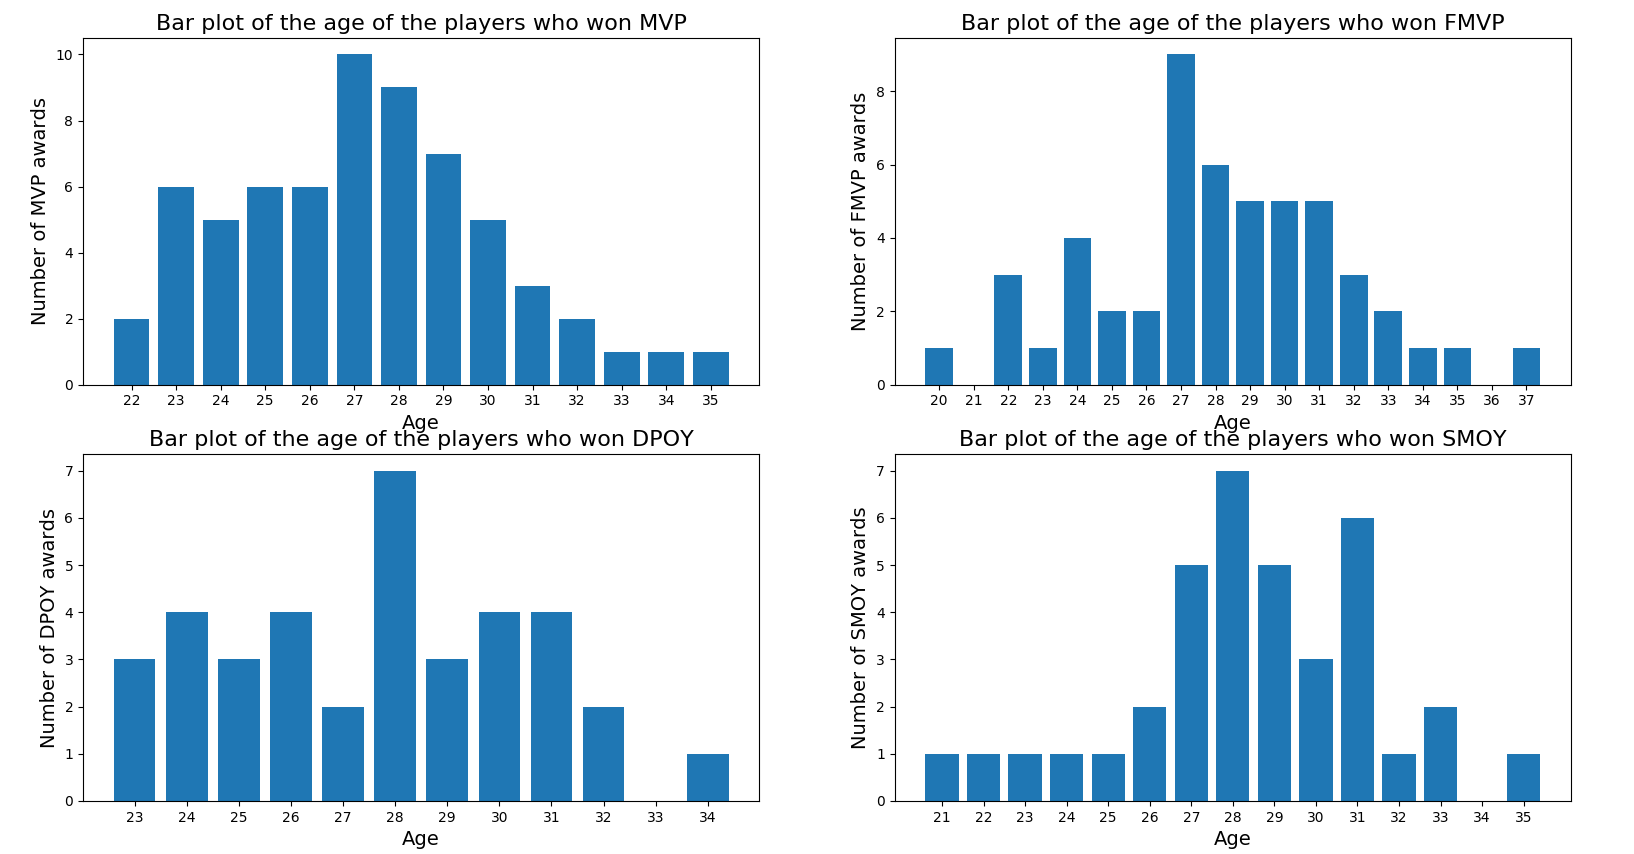
\includegraphics[scale=0.3]{awards_plots.png}
\end{center}
\caption{Age of award winners}
\label{plt:awards}
\end{figure}

First, I checked age of players who played in the NBA. Results can be seen in histogram (figure \ref{plt:age_hist}). Note that there are two histograms. One represents every player who played in the NBA (in the three point era, from 1979/80 season). The other is filtering out every player (from the same era) that has played in less than 25 games and less then 15 minutes per game. Those players are filtered because I don't consider them regular contributors for the team they are playing for, so they might not be important. Also, I just wanted to check on their histogram as well.  

\begin{figure}[h!]
\begin{center}
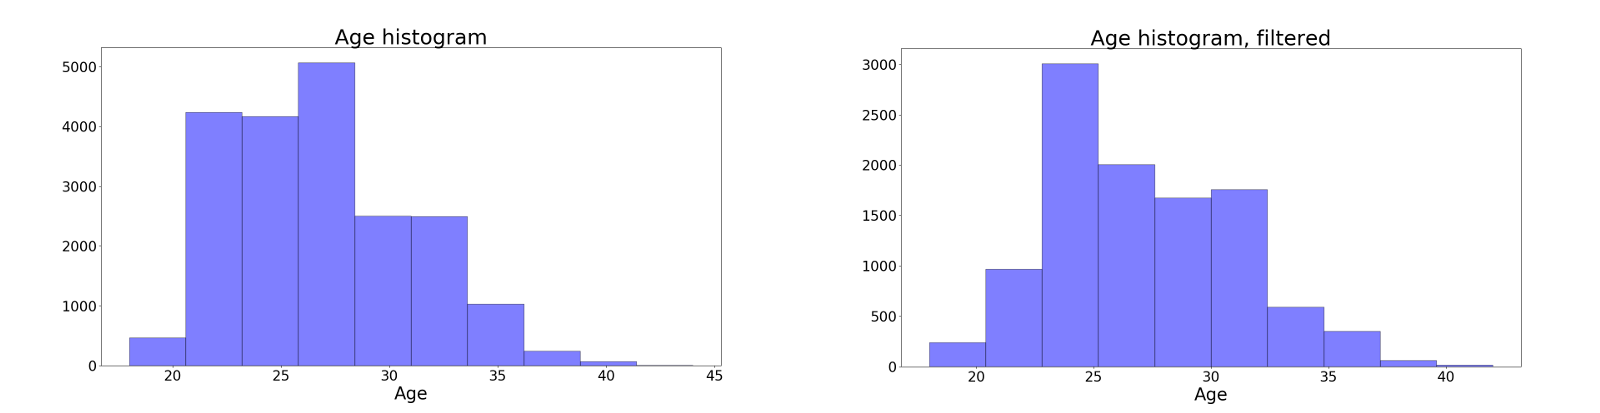
\includegraphics[scale=0.3]{age_histograms.png}
\end{center}
\caption{Age histograms}
\label{plt:age_hist}
\end{figure}


TODO -> comment about age histograms, and then show other plots


\pagebreak

\addcontentsline{toc}{section}{References}
\appendix
\bibliography{ref}
\bibliographystyle{unsrt}
\appendix

\end{document}
